\section{Trabajo realizado a lo largo de Trabajo Terminal II}

\noindent
En el presente apartado se muestra el trabajo realizado durante el periodo de Trabajo Terminal II, el cual consideramos a partir de la segunda mitad del mes de Mayo del presente año, hasta diciembre del mismo. Las iteraciones contempladas para el referido son 13, mismas cuya distribución se pueden observar en el esquema debajo, mismo que muestra también el contraste con las iterciones consideradas en el trabajo terminal I.

\begin{figure}[!htpb]
	\hypertarget{fig:iteraciones}{\hspace{1pt}}
	\begin{center}
		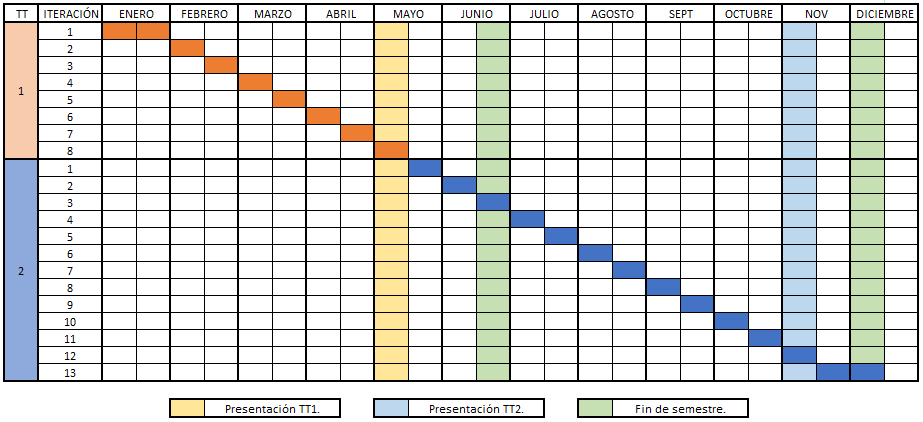
\includegraphics[width=1\textwidth]{images/reporte/iteraciones.png}
		\caption{Iteraciones realizadas a lo largo de TT1 y TT2.}
		\label{fig:iteraciones}
	\end{center}
\end{figure}

\noindent
A continuación, se describen cada una de las iteraciones realizadas en el periodo de Trabajo Terminal II.

\subsection{Primera iteración}

\noindent
\textbf{Objetivo}: Replantear estructura de los módulos para Bolsa de trabajo.
\newline

\noindent
\textbf{Descripción}: En esta primera iteración se revisa la modularización del sistema, ya que, a petición del uno de lo sinodales, se debía de reconsiderar la forma en que se estaba manejando el módulo de web bolsa. Por lo que se decide revisar de nuevo la planeación, el anális y diseño de lo trabajado en TTI, de donde se realizan unos primeros cambios al módulo de web bolsa. Sin embargo, las consideraciones que se tenían para el antes mencionado eran bastantes, por lo que se rediseña por completo el módulo, dando paso a la eliminación de éste y a la creación de dos nuevos módulos referentes a la bolsa de trabajo: Bolsa web y Alumno bolsa. 
\newline
\newline
Para ello, se realizan investigaciones sobre la bolsa de trabajo y la forma en que las empresas logran ofertar empleos a través de esta última. Se obtiene información de SIBOLTRA, de su estructura, y de la forma que trata a las ofertas laborales. Con la información recabada, nos percatamos que no es el enfoque que la aplicación o la comunidad ESCOM requería, pues, a pesar de ser el origen de ello, no era necesario trabajar desde ese punto de vista, sino obtener la información directamente de la propia ESCOM por medio del departamento de extensión y apoyos educativos, debido a que es el propio encargado del mencionado quien se encarga de realizar el proceso de registro de empresas para ofertar empleos, de recibir las propuestas, de llevar el control de las mismas, de generar boletines con la información obtenida y de publicar el mismo por medio de sus redes sociales (asociadas al departamento). Así bien, se decide acudir con el encargado del departamento antes mencionado, presentarle el proyecto, comentarle de la idea postulada para los módulos de bolsaWeb y alumnoBolsa e invitarle a colaborar en el desarrollo de éstos, teniendo una respuesta entusiasta y positiva al respecto. 
\newline
\newline
Fue así, que comenzamos a tener juntas con José Francisco Serrano García (actual encargado del departamento de extensión y apoyos educativos), con el fin de obtener información detallada acerca de los procesos que éste realiza para hacer llegar la información de las ofertas de trabajo de la bolsa de trabajo a los alumnos y comunidad en general de la ESCOM. Una vez obtenida dicha información, proseguimos con el análisis y el diseño (en maquetado) del módulo de Bolsa web, mismo que se pensó para uso de Francisco, en sustitución de todos los procesos que él realiza para compartir la información de la bolsa de trabajo en ESCOM. Los casos de uso obtenidos para este módulo son 10 y giran en torno al registro, edición, eliminación y consulta de las empresas y ofertas de trabajo en el sistema web que se diseña para cubrir este aspecto. 
\newline
Concretamente, para esta iteración, el trabajo realizado fue: 
\begin{itemize}
	\item Replanteamiento de la modularización del sistema, obteniendo dos primeros y nuevos módulos centrados en la bolsa de trabajo en ESCOM: bolsaWeb y alumnoBolsa.
	\item Investigación sobre SIBOLTRA y la bolsa de trabajo en el IPN.
	\item Investigación sobre procesos realizados en el departamento de extensión y apoyos educativos para los procesos en torno a la bolsa de trabajo.
	\item Toma de requisitos con encargado del departamento para generar propuestas.
	\item Identificación de casos de uso para el módulo bolsaWeb.
	\item Diseño de maquetas sobre el módulo mencionado.
\end{itemize}

% *************** S E G U N D A   I T E R A C I Ó N. *************** %

\subsection{Segunda iteración}

\noindent
\textbf{Objetivo}: Presentar propuestas de solución para nuevos módulos de Bolsa de Trabajo.
\newline

\noindent
\textbf{Descripción}: Para la segunda iteración se presenta la propuesta de pantallas al licenciado Francisco, se obtiene retroalimentación del mismo y se corrigen o añaden a las pantallas los puntos importantes tomados de las observaciones mencionadas. Con ello, se comienza la redacción de los nuevos casos de uso para el módulo de bolsaWeb, con sus respectivas reglas de negocio y mensajes.
\newline
\newline
Por otro lado, de manera casi paralela, se empieza el desarrollo del módulo como página web, para el cual se requirieron tecnologías y herramientas tales como HTML5, CSS, php, MySQL, Java Script, JQuery, JSON, entre otros. Teniendo así la creación del servidor de la app. Es importante mencionar que para el desarrollo del servidor, del cliente (vistas del sistema para Francisco) y demás aspectos relevantes como la base de datos, se debieron conocer la forma en que los servidores de ESCOM podrían alojar a la aplicación, pues, gracias a pláticas con nuestros directores y el director de la ESCOM, licenciado Andrés Ortigoza, se determinó que la app podría ser huésped en la propia ESCOM y sus servidores, así bien, una vez conocida la información de los servidores, la base de datos, entre otros, de la superior de cómputo y cómo es que éstos trabajan, se procede a reestructurar la base de datos de ESCOMobile, adaptándola al nuevo negocio de la bolsa de trabajo, además de hacer pruebas con JSON para el envío de información en el sistema.
\newline
Es entonces que se presenta un primer prototipo del sistema web al licenciado Serrano y se recibe, de nueva cuenta, retroalimentación sobre el sistema, la información manejada y la forma en que es compartida. 
\newline
El avance concreto obtenido en esta iteración fue: 
\begin{itemize}
	\item Realización de correcciones y agregados en el modelado de maquetas para bolsaWeb.
	\item Investigación sobre posibles formas de realizar y alojar el servidor de ESCOMobile.
	\item Investigación acerca de los servidores de ESCOM y cómo trabajan.
	\item Adaptación de la base de datos a los nuevos requerimientos.
	\item Pruebas con JSON para el envío de información.
	\item Redacción de reglas de negocio y mensajes para módulo bolsaWeb.
	\item Redacción de casos de uso del módulo mencionado.
	\item Desarrollo de servidor de ESCOMobile.
	\item Realización de página web dedicada a la bolsa de trabajo en ESCOM.
\end{itemize}

% *************** T E R C E R A   I T E R A C I Ó N. *************** %

\subsection{Tercera iteración}

\noindent
\textbf{Objetivo}: Presentar prototipo de los nuevos módulos del sistema: alumnoBolsa y bolsaWeb.
\newline

\noindent
\textbf{Descripción}: En este periodo de tiempo se continuó trabajando sobre el sistema web referente al módulo bolsaWeb de ESCOMobile, corrigiendo, primeramente, las observaciones realizadas en las juntas con el encargado del departamento de extensión y apoyos educativos, agregando además detalles sobre el registro de ofertas y empresas, que permiten facilitar el trabajo del encargado del departamento. 
\newline
Es aquí cuando se agregan al sistema web nuevos e interesantes aspectos, como el inicio de sesión en el sistema por medio de Facebook, la generación automática de boletines de ofertas de trabajo y la publicación también automática de éstos en Facebook gracias al previo inicio de sesión y su conexión con ESCOMobile.
\newline
\newline
Además, es cuando se comienza con el análisis y diseño del segundo módulo la bolsa de trabajo: alumnoBolsa. Un módulo dedicado a la aplicación móvil, con el cual alumnos y profesores de la ESCOM que utilicen la app, podrán consultar las ofertas de trabajo registradas y publicadas, directamente desde la app en un smartphone. Se realizan pantallas del módulo y se comienza con la redacción de reglas de negocio, mensajes y casos de uso para el mismos.
\newline
Con lo anterior, se tenía casi cubierto el aspecto de bolsa de trabajo, solicitado por el profesor Asunción, dando pie al desarrollo de la app ESCOMobile tal cual se tenía planeado. 
\newline
Para esta iteración el avance que se obtuvo fue el siguiente:
\begin{itemize}
	\item Realización de correcciones y agregados en el modelado de maquetas para bolsaWeb.
	\item Investigación e implementación sobre inicio de sesión al sistema por medio de Facebook.
	\item Generación automática de boletines como añadido al sistema. 
	\item Publicación automática de boletines en Facebook, como segundo añadido.
	\item Identificación de casos de uso para módulo alumnoBolsa.
	\item Análisis, diseño y construcción de maquetas para el referido.
	\item Redacción de reglas de negocio, mensajes y casos de uso para alumnoBolsa.
\end{itemize}

% *************** C U A R T A   I T E R A C I Ó N. *************** %

\subsection{Cuarta iteración} 

\noindent
\textbf{Objetivo}: Reorganizar estructura de módulos que componen ESCOMobile, replanteando el negocio.
\newline

\noindent
\textbf{Descripción}: Para la presente se hacen correcciones al módulo bolsaWeb quedando en una versión beta, al estar revisada por el licenciado Francisco. Así nos concentramos en la implementación del su módulo hermano, alumnoBolsa, con el cual se pretende llevar las ofertas de trabajo previamente publicadas a los alumnos de ESCOM por medio de ESCOMobile. Así, se desarrolla el módulo descrito, se presenta a directores y encargado del departamento y se obtienes observaciones al respecto, por ejemplo, que no solo se consulten la información de las ofertas de trabajo en el sistema, sino tener interacción entre el smartphone y el usuario quien consulta las anteriores, pues es posible usar la propia consulta como punto de extensión para contactar a la empresa que oferta el empleo. 
\newline
\newline
Por otro lado, una vez obtenida retroalimentación para el módulo de alumnoBolsa, se comienzan a reorganizar los nueve módulos restantes que componían a ESCOMobile y que fueron dados a conocer durante la presentación de TT1, pues gracias a los comentarios de directores y sinodales, nos percatamos que el enfoque que se le había dado no era el mejor. Es entonces que se vuelve a analizar el diseño y el alcance propuesto para ESCOMobile, se ajustan ciertos aspectos y se realizar una reestructuración completa en la planeación del sistema, siempre respetando los objetivos del proyecto y la esencia del mismo, así como los objetivos y los resultados prometidos.
\newline
Es aquí donde se plantea desde cero la estructura de la app, completando los dos módulos previamente realizados y modificando, expandiendo y mejorando los primeros dos presentados durante TT1 (acceso y mapa), de donde, ahora se cuenta con 8 módulos para la app, resultado de nuevo profundo análisis realizado. Los módulos considerados dentro de ESCOMobile son: Acceso, Mapa, Alumno, AlumnoBolsa, AlumnoProfesor, Profesor, Citas y BolsaWeb. Siendo cada uno de ellos muy concreto y específico con respecto al rol que juegan en el sistema y lo que permiten hacer a los actores dentro del mismo. 
\newline
Por último, en esta iteración, se presenta la nueva estructura a directores y sinodales, mismos que concordaron ante ella y se comenzó la planeación del análisis, diseño, desarrollo e integración de los nuevos módulos al sistema.
\newline
A continuación se muestran los módulos que componían a ESCOMobile, así como los nuevos módulos que dan vida al sistema. 
\begin{figure}[!htpb]
	\hypertarget{fig:reestructuracion}{\hspace{1pt}}
	\begin{center}
		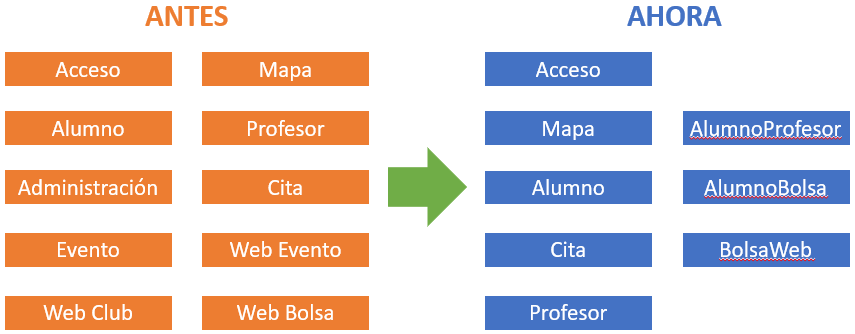
\includegraphics[width=1\textwidth]{images/reporte/reestructuracion.png}
		\caption{Comparativa entre estructuras de ESCOMobile y sus módulos.}
		\label{fig:reestructuracion}
	\end{center}
\end{figure}

\noindent
De lo anterior, podemos observar que durante este periodo de tiempo se pudo trabajar en:
\begin{itemize}
	\item Realización de correcciones y agregados en el modelado de maquetas para bolsaWeb.
	\item Desarrollo del módulo alumnoBolsa.
	\item Revisión de protocolo, análisis, diseño e implementación de trabajo en TT1.
	\item Reestructuración de los módulos en ESCOMobile.
\end{itemize}

% *************** Q U I N T A   I T E R A C I Ó N. *************** %

\subsection{Quinta iteración} 

\noindent
\textbf{Objetivo}: Presentar prototipo de la app presentado en TT1 (módulos de acceso y mapa) con correcciones y añadidos. 
\newline

\noindent
\textbf{Descripción}: Durante la quinta iteración se realizaron correcciones en el módulo de alumnoBolsa y se presenta un nuevo prototipo de éste. Además, se retoman primeramente los dos primeros módulos de la nueva estructura de ESCOMobile, éstos son Acceso y Mapa, para su adaptación al nuevo modelo del sistema. Se reescriben más adelante por completo los casos de uso correspondientes a los anteriores, con sus respectivas reglas de negocio y mensajes.
\newline
En esta iteración se vuelven a tomar fotografías de la ESCOM y se realizan nuevos bocetos para completar los pisos restantes de la institución para su digitalización, además se realiza diseño de logo para el sistema. Posteriormente, una vez obtenido lo anterior se procede a digitalizar los mapas y logo para su implementación dentro del sistema. Y se redactan los términos y condiciones que el usuario debe aceptar para poder ser registrado en el sistema y utilizar los servicios que éste le brinda. 
\newline
\newline
Además, se realizan maquetas para los 4 módulos que no tenían el diseño en maquetado, éstos son: Alumno, AlumnoProfesor, Profesor y Citas, y se rediseñan las propias para los módulos de acceso y mapa, adaptándolos al nuevo modelo propuesto. 
\newline
Es entonces que se comienza con la adaptación de diseño y redacción de casos de uso, reglas de negocio y mensajes para los nuevos casos de uso en los módulos de acceso y mapa, permitiéndonos además completar el desarrollo de los mismos en sus casos de uso de alta prioridad, ya con la implementación de los nuevos mapas y el desarrollo de la búsqueda de profesores, para la cual se tuvo que investigar y realizar una conexión entre nuestra base de datos y la vista proporcionada por el licenciado Ortigoza con la información de los profesores en ESCOM, sus horarios, clases y salones.
\newline
Finalmente, en esta iteración, se integra todo lo anterior en la aplicación móvil de ESCOMobile y se presenta prototipo a directores y sinodales.
\newline
A continuación se muestran algunas de las pantallas diseñadas para el sistema, para los módulos de la nueva estructura propuesta para ESCOMobile. 
\begin{figure}[!htpb]
	\hypertarget{fig:interfaces_uno}{\hspace{1pt}}
	\begin{center}
		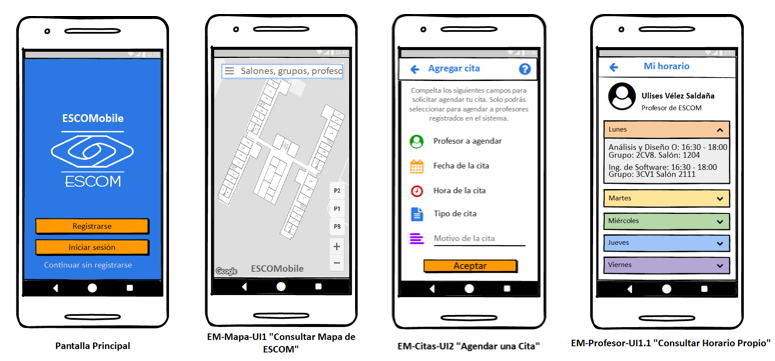
\includegraphics[width=1\textwidth]{images/reporte/interfaces1.png}
		\caption{Diseño de algunas pantallas de módulos para ESCOMobile A.}
		\label{fig:interfaces_uno}
	\end{center}
\end{figure}

\begin{figure}[!htpb]
	\hypertarget{fig:interfaces_dos}{\hspace{1pt}}
	\begin{center}
		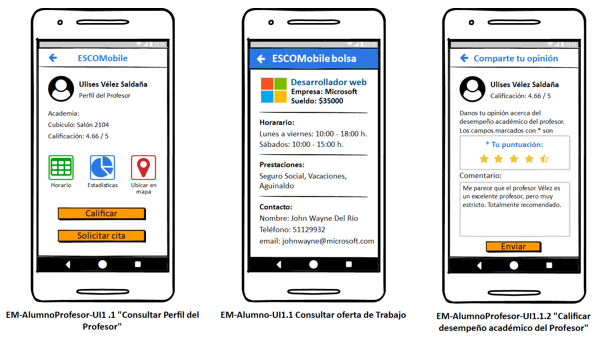
\includegraphics[width=1\textwidth]{images/reporte/interfaces2.png}
		\caption{Diseño de algunas pantallas de módulos para ESCOMobile B.}
		\label{fig:interfaces_dos}
	\end{center}
\end{figure}

Así, se tiene que el trabajo realizado para esta iteración es: 
\begin{itemize}
	\item Realización de correcciones y agregados para el módulo de alumnoBolsa.
	\item Adaptación de los módulos de acceso y mapa al nuevo modelo.
	\item Realización de bocetos para los mapas restantes y logo de la aplicación.
	\item Redacción de los términos y condiciones para poder registrarse en el sistema.
	\item Diseño de maquetas para los módulos Alumno, AlumnoProfesor, Profesor y Citas.
	\item Rediseño de pantallas para los módulos de acceso y mapa, además de creación de pantallas para los nuevos casos de uso que se agregaron a los antes mencionados.
	\item Redacción de reglas de negocio, mensajes y casos de uso para los rediseñados casos de uso de acceso y mapa.
	\item Conexión de base de datos con vista otorgada con la información de los profesores.
	\item Desarrollo de los módulos acceso y mapa con búsqueda de profesores integrada.
	\item Entrega de prototipo.
\end{itemize}

% *************** S E X T A   I T E R A C I Ó N. *************** %

\subsection{Sexta iteración}

\noindent
\textbf{Objetivo}: Analizar y diseñar módulos alumno, alumnoProfesor, profesor y citas, pertenecientes a la nueva estructura del sistema.
\newline

\noindent
\textbf{Descripción}: Para esta sexta iteración se corrigieron detalles y observaciones sobre el prototipo entregado anteriormente, dejando los primeros módulos desarrollados del sistema (acceso, mapa, bolsaWeb y alumnoBolsa) en estado de beta. Así se comenzaron a redactar las reglas de negocio, mensajes y casos de uso para los dos siguientes módulos: alumno y profesor. Por otro lado, se comienza la redacción de los guiones de prueba de los módulos bolsaWeb y alumnoBolsa, mismos que contemplan posibles situaciones ante las cuales la aplicación puede estar expuesta (en estos módulos), con el fin de localizar errores, que no se pueden presentarse en el uso cotidiano de la misma, y corregirlos.
\newline
Por otra parte, se comienza con la redacción de la documentación técnica, misma que se redacta desde cero, pues el nuevo negocio lo requería de esa manera. Para esta iteración se redactó la introducción, la justificación, el estado del arte y el maco teórico.
\newline
Debajo se muestra un fragmento de uno de los guiones de prueba, como ejemplo del comienzo de la redacción de los mismos. 
\begin{figure}[!htpb]
	\hypertarget{fig:guion_prueba}{\hspace{1pt}}
	\begin{center}
		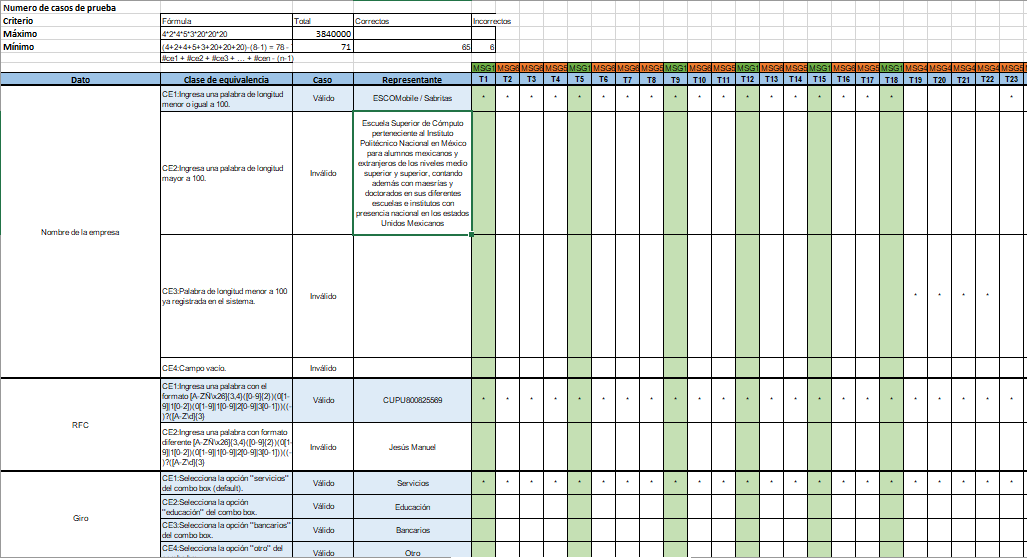
\includegraphics[width=1\textwidth]{images/reporte/guionPrueba.png}
		\caption{Fragmento de guión de prueba para el módulo de bolsaWeb.}
		\label{fig:guion_prueba}
	\end{center}
\end{figure}

De tal forma, que el trabajo concreto realizado durante esta iteración fue:
\begin{itemize}
	\item Realización de correcciones y agregados para el prototipo anterior.
	\item Redacción de reglas de negocio y mensajes para los módulos alumno y profesor.
	\item Redacción de los casos de uso para los anteriores.
	\item Redacción de guiones de prueba para los módulos de bolsaWeb y alumnoBolsa.
	\item Comienzo de documentación técnica, contemplando introducción, justificación, estado del arte y maco teórico.
\end{itemize}


% *************** S É P T I M A   I T E R A C I Ó N. *************** %

\subsection{Séptima iteración}

\noindent
\textbf{Objetivo}: Entregar prototipo con los módulos de alumno y profesor programados y los módulos bolsaWeb y alumnoBolsa probados.
\newline

\noindent
\textbf{Descripción}: Durante la presente iteración nos concentramos en 4 cosas principales: Análisis y diseño, desarrollo, pruebas y redacción del documento. A continuación, se describen brevemente cada uno de estos apartados.
\newline
\newline
Para el análisis y el diseño se consideró la redacción de los casos de uso correspondientes al módulo de alumnoProfesor, conteniendo en éste las reglas de negocio y mensajes necesarios para la realización del mismo, así como la descripción de sus pantallas y la revisión de los propios. Pues, es necesario entregar un buen trabajo en los mencionados, ya que son base para su desarrollo próximo.
\newline
\newline
Para el desarrollo, en esta iteración se consideró el módulo de alumno y profesor, en sus casos de uso de alta prioridad. Considerando la investigación e implementación de nuevos conocimientos para su realización. Es aquí cuando se entrega un nuevo prototipo a los directores y sinodales, completando ya gran parte de la aplicación en beta. El entusiasmo del jurado fue tal, que se nos pidió alojáramos la app en un servidor para ser accedida desde cualquier punto por cualquier persona, pues, hasta ahora no se había realizado de esta forma, observación que se aprecia y se implementaría posteriormente. Ellos nos sugirieron en la propia ESCOM.
\newline
\newline
Para el apartado de pruebas, se comienzan a realizar las pruebas para los módulos de bolsaWeb y alumnoBolsa, tomando como referencia los guiones previamente escritos, por tanto, se crea también un archivo (en este caso en la nube) para escribir y atender incidencias en el sistema, obtenidas gracias a las pruebas realizadas. 
\newline
Asimismo, se comienza la redacción de guiones de prueba para los módulos de acceso y mapa, basados en sus propios casos de uso. 
\newline
\newline
Finalmente, se continúa con la redacción del documento, esta vez acoplando al mismo los casos de uso previamente escritos y agregando objetivos, problemática, tecnologías a usar e identificación de requerimientos funcionales y no funcionales.
\newline
Así, para esta iteración el trabajo realizado se menciona a continuación:
\begin{itemize}
	\item Redacción de reglas de negocio y mensajes para el módulo alumnoProfesor.
	\item Redacción de los casos de uso para el anterior.
	\item Desarrollo de los módulos alumno y profesor.
	\item Redacción de guiones de prueba para los módulos de mapa y acceso.
	\item Pruebas para los módulos bolsaWeb y alumnoBolsa.
	\item Redacción de objetivos, problemática, tecnologías a usar e identificación de requerimientos funcionales y no funcionales en la documentación técnica.
	\item Entrega de prototipo del sistema hasta los módulos programados.
\end{itemize}

% *************** O C T A V A   I T E R A C I Ó N. *************** %

\subsection{Octava iteración}

\noindent
\textbf{Objetivo}: Entregar prototipo con el módulo de alumnoPofesor programado y los módulos acceso y mapa probados. Buscar alojamiento de la app en los servidores de ESCOM. 
\newline

\noindent
\textbf{Descripción}: En esta iteración, al igual que en la anterior, el trabajo se dividió principalmente en cuatro aspectos, los cuales son: Análisis y diseño, desarrollo, pruebas y redacción del documento. De bajo se hace una breve descripción de la manera en que se enfocó cada uno de estos aspectos en el trabajo a entregar.
\newline
\newline
En el apartado del análisis y el diseño se trabajó principalmente con el módulo de citas, un módulo de especial importancia en la aplicación, pues al igual que el mapa, es uno de los más grandes atractivos en la app. Así, se comienza el análisis y diseño, contemplando la redacción de sus correspondientes casos de uso, incluyendo con éstos la redacción de las reglas de negocio y mensajes necesarios para la realización de los mismos, así como la descripción de sus pantallas y la revisión de los propios. 
\newline
\newline
En el aspecto del desarrollo, se realizan primeramente las correcciones de las incidencias encontradas anteriormente. Se comienza con la implementación del módulo alumnoProfesor, mismo que también es de suma importancia en el sistema, pues, permite interactuar a los alumnos y profesores por medio de la consulta de la información de los mismos, así como brindar sus opiniones acerca del desempeño que los docentes tienen en la Superior de cómputo desempeñando su labor. Los casos de uso contemplados son, de nueva cuenta, los de alta prioridad. Considerando la investigación e implementación de nuevos conocimientos para su realización. Teniendo al finalizar el desarrollo del presente módulo un nuevo prototipo. 
\newline
Por otro lado, se contemplan aspectos que serán necesarios en el desarrollo futuro, como lo son las notificaciones en la aplicación, mismas que son usada en el módulo de citas, por ejemplo. Por lo que se comienza a investigar al respecto y a realizar pruebas con ellas. 
\newline
Además, se realiza la petición del servidor en ESCOM para alojar la aplicación en el mismo, la atención brindada por el profesor Antonio fue muy grata en todo momento, cooperó gustosamente con el proyecto, por lo cual se preparó todo para alojar parte del sistema en el servidor de la escuela.
\newline
\newline
En el aspecto de las pruebas, se realizan las mismas para los módulos de acceso y mapa, tomando como referencia los guiones previamente escritos. Asimismo, se comienza la redacción de guiones de prueba para los módulos de alumno y profesor, basados en sus respectivos casos de uso. 
\newline
\newline
Por último, continuamos agregando aspectos a la documentación técnica del sistema, como lo son, descripción de los módulos, sus casos de uso y diagramas de casos de uso.
\newline
De donde, el trabajo obtenido a lo largo de esta iteración fue:
\begin{itemize}
	\item Corrección de incidencias encontradas.
	\item Redacción de reglas de negocio y mensajes para el módulo de citas.
	\item Redacción de los casos de uso para el anterior.
	\item Desarrollo del módulo alumnoProfesor.
	\item Redacción de guiones de prueba para los módulos de alumno y profesor.
	\item Pruebas para los módulos acceso y mapa e incidencias para los mismos.
	\item Redacción de módulos y diagramas de casos de uso dentro de la documentación técnica.
	\item Pruebas con notificaciones dentro de Android.
	\item Petición de alojamiento de ESCOMobile en los servidores de ESCOM.
	\item Preparación y alojamiento de la app en ESCOM.
	\item Entrega de prototipo del sistema hasta los módulos programados.
\end{itemize}

% *************** N O V E N A   I T E R A C I Ó N. *************** %

\subsection{Novena iteración} 

\noindent
\textbf{Objetivo}: Entregar prototipo con el módulo de citas programado y el módulo de alumnoProfesor probado.
\newline

\noindent
\textbf{Descripción}: Al igual que las iteraciones anteriores, la presente se enfoca en los cuatro puntos anteriormente tratados, los cuales son análisis y diseño, desarrollo, pruebas y documentación. En seguida se describe el trabajo realizado en este periodo de tiempo para cada uno de estos apartados. 
\newline
\newline
Para el primero de los mencionados se realizó una completa revisión del módulo de citas, pues, como ya hemos mencionado, lo consideramos pilar de la aplicación. 
\newline
\newline
Para el apartado de desarrollo, se trabaja con las correcciones de incidencias encontradas en la iteración anterior. Y se comienza con la implementación del módulo de citas, teniendo muchos aspectos a considerar durante el mismo, como la interacción propia que tienen los actores para con el sistema, el envío de notificaciones y el tratado de las citas para con los actores. Asimismo, con el apartado de ''agendar citas'', para dar paso a un completo módulo de citas disponible para la app. 
\newline
Para este momento del trabajo ya se cuenta con la aplicación en el servidor, por lo que puede ser accedida desde cualquier parte en cualquier momento, con el simple hecho de instalar el APK de la misma. Así, de comienza la distribución de la app con nuestros amigos cercanos de ESCOM que cuenten con un smartphone android, para que puedan ir probándola y dar su opinión como usuarios directos. 
\newline
\newline
En el aspecto de las pruebas, se realizan las mismas para los módulos de alumno y profesor, tomando como referencia los guiones previamente escritos. Asimismo, se comienza la redacción de guiones de prueba para el módulo de alumnoProfesor, basados en sus respectivos casos de uso. 
\newline
Además, para el documento técnico del sistema, se empiezan a tener correcciones acerca de la forma en que se redactó y faltas en la ortografía, por lo que se inicia a depurar el mismo, de estos errores.
\newline
\newline
Finalmente, debe mencionarse, que durante esta iteración se realzaron cambios importantes en el equipo detrás de ESCOMobile, pues uno de los integrantes del equipo decidió no participar más en el mismo, debido a la gran carga de trabajo, siendo su parte (digitalización de mapas) retirada de la aplicación. 
\newline
Así bien, lo acontecido durante esta iteración se describe a continuación. 
\begin{itemize}
	\item Corrección de incidencias encontradas.
	\item Revisión de análisis y diseño para citas.
	\item Desarrollo del módulo citas.
	\item Redacción de guiones de prueba para el módulo de alumnoProfesor.
	\item Pruebas para los módulos alumno y profesor e incidencias para los mismos.
	\item Corrección de documento técnico del sistema.
	\item Reorganización del equipo de ESCOMobile.
	\item Entrega de prototipo del sistema hasta los módulos programados.
\end{itemize}

% *************** D É S I M A   I T E R A C I Ó N. *************** %

\subsection{Décima iteración}

\noindent
\textbf{Objetivo}: Realizar pruebas generales en el prototipo presentado.
\newline

\noindent
\textbf{Descripción}: Para el momento en que transcurría esta iteración la presentación de Trabajo Terminal II estaba muy próxima, por lo que debíamos concentrarnos en el trabajo que se iba a presentar, haciéndolo de la mejor manera posible. Así, para la presente se realizó el siguiente trabajo. 
\newline
\newline
Se trabaja en probar de nueva cuenta la aplicación en los módulos anteriores para encontrar más incidencias, a parte de las ya encontradas en iteraciones pasadas. Se comienzan a corregir aspectos generales de la app, como íconos, colores de pantallas, etc. Además, se realizan nuevos mapas de ESCOM para la app, gracias al apoyo de una diseñadora gráfica.
\newline
En el aspecto de las pruebas, se realizan las mismas para el módulo de alumnoProfesor, tomando como referencia los guiones previamente escritos. Asimismo, se comienza la redacción de guiones de prueba para el módulo de citas, basados en sus respectivos casos de uso. 
\newline
Además, para el documento técnico del sistema, se continúan con correcciones acerca de redacción, ortografía y apartados generales del mismo.
\newline
Así bien, lo acontecido durante esta iteración se describe a continuación. 
\begin{itemize}
	\item Corrección de incidencias encontradas.
	\item Pruebas generales de la app. 
	\item Redacción de guiones de prueba para el módulo de citas.
	\item Pruebas para los módulos alumnoProfesor e incidencias para los mismos.
	\item Corrección de documento técnico del sistema.
	\item Entrega de prototipo del sistema hasta los módulos programados.
\end{itemize}

% *************** O N C E A V A   I T E R A C I Ó N. *************** %

\subsection{Decimoprimera iteración}

\noindent
\textbf{Objetivo}: Entregar documentación del sistema y prototipo corregido.
\newline

\noindent
\textbf{Descripción}: Para esta iteración se comienza, principalmente, a organizar todo lo referente a la presentación de trabajo terminal II. Se continúan haciendo correcciones a la documentación técnica del sistema, y se comienza la redacción del presente reporte final de trabajo, que incluye, entre otras cosas, antecedentes del trabajo, trabajo realizado, resultados y trabajo a futuro.
\newline
\newline
Se continúa probando el sistema, con especial énfasis en el módulo de citas, tomando como referencia los guiones previamente escritos. Además, se corrigen incidencias y se comienza a mostrar avances generales del sistema a los directores y sinodales, se empiezan a obtener las firmas para poder presentar. Se considera la distribución de la app, para lo cual se tienen citas con el licenciado Ortigoza, mismo que se encuentra involucrado en el proceso.  
\newline
Así, el trabajo que se realizó a lo largo de la presente fue:
\begin{itemize}
	\item Corrección de incidencias encontradas.
	\item Pruebas generales de la app. 
	\item Corrección de documento técnico del sistema.
	\item Redacción de reporte final de trabajo.
	\item Pruebas para el módulo de citas.
	\item Corrección de documento técnico del sistema.
	\item Entrega de avances generales a directores y sinodales.
\end{itemize}

% *************** D O C E A V A   I T E R A C I Ó N. *************** %

\subsection{Decimosegunda iteración} 

\noindent
\textbf{Objetivo}: Preparar diapositivas, publicidad, comerciales, etc. del sistema para presentación de TT2.
\newline

\noindent
\textbf{Descripción}: La presente iteración es la iteración final, por lo que el trabajo que se realizó se concentra en correcciones del sistema, así como en los documentos técnico y reporte, agregando a éstos ciertos detalles y afinando otros. Se comienza la realización de las diapositivas a usar en la presentación, así como videos ilustrativos del sistema, cómo funciona y lo que ofrece. Se realizan presentaciones prueba con directores y se organiza estructura de la presentación, así como los detalles que a ésta acompañan.
Se realiza proceso previo a la presentación con los diferentes departamentos de la ESCOM. 
\newline
El trabajo realizado para esta iteración fue:
\begin{itemize}
	\item Corrección de incidencias encontradas.
	\item Pruebas generales de la app. 
	\item Corrección de documento técnico del sistema y reporte final.
	\item Realización de diapositivas para presentación.
	\item Realización de video ilustrativo del sistema.
	\item Proceso previo a presentación.
\end{itemize}

% *************** D O C E A V A   I T E R A C I Ó N. *************** %

\subsection{Decimotercera iteración} 

\noindent
\textbf{Objetivo}: Corregir y añadir aspectos obtenidos de observaciones realizadas por sinodales durante la presentación de TT2.
\newline

\noindent
\textbf{Descripción}: Para esta iteración de tiene planeado analizar y, según sea el caso, realizar las correcciones propuestas por directores y sinodales acerca del sistema y la documentación mostrados durante la presentación de TT2. Así como continuar con los detalles finales de la aplicación, como programación y pruebas a casos de uso de baja prioridad. Probar de nueva cuenta el sistema general para obtener nuevos fallos dentro del mismo, para su próxima corrección. Implementación del sistema en la ESCOM, comenzando así con las actividades descritas en el capítulo de ''trabajo a futuro'', contenido en el presente documento. 
\newline
Así, el trabajo propuesto para esta iteración es:
\begin{itemize}
	\item Atención de observaciones del jurado hacia el sistema y su documentación, realizadas durante la presentación de TT2.
	\item Desarrollo de casos de uso de prioridad baja.
	\item Pruebas generales de la app. 
	\item Planeación y organización para cumplir con las tareas descritas en la sección de trabajo a futuro.
\end{itemize}


% ************************************************************************ %
% ***********     R E S U L T A D O S   O B T E N I D O S.     *********** %
% ************************************************************************ %

\section{Resultados obtenidos durante el Trabajo Terminal II}

\noindent
A lo largo del Trabajo Terminal II se realizaron modificaciones, avances, reestructuraciones y demás aspectos que definieron el actual estado de ESCOMobile. Durante 6 meses, desde que terminó la presentación de TT1 y hasta la actual fecha, nos hemos dedicado a que el sistema crezca, cumpla con lo prometido y sea útil para quien lo utilice. Es así que nos dedicamos al desarrollo de la app, basada en una organización que se planeó y detalló de la mejor forma. Gracias a los casos de uso redactados, pruebas y observaciones de directores y sinodales es posible que hoy exista la app que comenzó como idea hace poco más de un año. 
\newline
A continuación, se describen los principales resultados que se obtuvieron del trabajo realizado a lo largo de TT2, separado por secciones para su fácil comprensión:
\newline
\newline
\textbf{Documentación}: Uno de los aspectos más importantes en un sistema software es la documentación del propio. Pues en ella se estipulan los aspectos técnicos del mismo. Además, sirve como modelo, pues, gracias a sus diagramas, descripciones, referencias, etc. se logra comprender la estructura y la manera en que el sistema se diseñó. Haciéndolo fácil de entender, expandir o modificar. Es por ello que la dedicación que le otorgamos cobró especial relevancia, redactando un documento técnico que contiene, entre otras cosas, introducción, justificación, objetivos, marco teórico, problemática, análisis y diseño, así como el modelado de las pantallas del sistema. Para la documentación técnica se contemplan también los casos de uso, siendo parte importante para el posterior desarrollo del sistema. Por otro lado, se redacta el documento referente al trabajo que se realizó a lo largo de Trabajo Terminal II, donde se incluyen los antecedentes del proyecto, como lo acontecido durante TT1, el trabajo realizado y los resultados obtenidos en TT2 y el trabajo a futuro para el sistema.
\newline
\newline
\textbf{Desarrollo de aplicación}: Para este apartado se realizó el desarrollo de la aplicación ESCOMobile, misma que contiene los ocho módulos descritos en el documento técnico del sistema, los cuales son: acceso, mapa, alumno, alumnoBolsa, alumnoProfesor, profesor, citas y bolsaWeb. La aplicación cuenta con un APK para poder ser instalada en cualquier dispositivo android, mismo que se puede descargar desde el siguiente enlace: \url{ http://www.comunidad.escom.ipn.mx/benjaminlb/download/}. Además, la app se encuentra alojada en los servidores de la Escuela Superior de Cómputo por lo que puede ser accedida siempre que éstos estén disponibles. Por otro parte, es importante mencionar que se han realizado pruebas al sistema, con el objetivo de minimizar los posibles errores que el usuario podría presenciar cuando la use, dichas prueban continúan y lo seguirán haciendo en el futuro, pues, es importante para nosotros hacer llegar al público un producto actualizado y de calidad. La app entregada cumple con lo prometido, permitiendo a alumnos y profesores esa interacción que facilita determinados procesos cotidianos de la ESCOM. Sin embargo, se tiene planeado expandir la misma en cuanto a funciones nos referimos. Además, se está buscando la manera de distribuirla en la ESCOM para su real uso en la misma.
\newline
\newline
Se debe mencionar que la aplicación, tal cual se encuentra hoy en día cumple con los objetivos marcados en el protocolo y con el resultado prometido a entregar. Debajo se especifica, en cada uno de los mencionados, cómo es que ESCOMobile cubre lo especificado.
\newline
\newline
\textbf{Objetivos}: Para asegurar el cumplimiento de ESCOMobile con los objetivos estipulados en el protocolo, debemos recordar los mismos, así, enlistamos los objetivos descritos: 
\begin{itemize}
	\item ''\textbf{General}: Desarrollar un sistema móvil que permita consultar la ubicación y disponibilidad de los profesores en la ESCOM, así como la consulta de áreas escolares dentro de ESCOM y diversos puntos de interés para el alumno, promoviendo un mayor aprovechamiento académico para el referido. 
	\item \textbf{Específicos}:
	\begin{itemize}
		\item Implementar motor de búsqueda de profesores, su disponibilidad y ubicación. 
		\item Proporcionar a alumnos de ESCOM e interesados información sobre las áreas académicas del plantel.
		\item Solucionar con tecnología móvil, simple, agradable e intuitiva la problemática de búsqueda y disponibilidad de profesores.''  
	\end{itemize}
\end{itemize}
De lo anterior, podemos decir que nuestra app cumple con el objetivo general, pues el sistema cuenta con el módulo de mapa, con el cual se pueden consultar las áreas de la ESCOM, distribuidas por pisos y edificios, permitiendo además realizar la búsqueda de los cubículos de los profesores, salones, grupos o academias dentro del plantel. 
\newline
En el caso de los objetivos específicos, debemos decir que se cumplen de igual forma, pues para cada uno de ellos tenemos un apartado dentro de la app. Para ser concretos, se tienen los módulos de alumnoProfesor para el primero de ellos, con el cual podemos, entre otras cosas realizar la búsqueda de profesores en ESCOM, ubicarlos en el mapa o bien, consultar sus horarios de clase; con ello se cubre el primero de los objetivos específicos. Para el segundo, presentamos el módulo de mapa, que, como ya dijimos para el objetivo general, permite consultar y ubicar áreas de la Superior de cómputo. Finalmente, para el tercer objetivo, se cuenta con un análisis y diseño de la aplicación que se cuidó y se orientó a que nos permita realizar las diferentes acciones que se nos permite dentro del sistema de una forma sencilla e intuitiva, tomando inspiración en el diseño de las aplicaciones de Android que se encuentran disponibles en la google play, además, se cuenta con el módulo de citas, con el cual pretendemos reducir el gasto innecesario de recursos para los alumnos, además de facilitar la comunicación académica de los alumnos con los profesores.
\newline
\newline
\textbf{Resultado esperado}: De igual forma, cuando se redactó y aceptó el protocolo que planteaba las bases a ESCOMobile y su desarrollo, se estipuló en un apartado dedicado el resultado esperado para entrega. A continuación, se muestra el fragmento referente al resultado esperado, tomado desde el protocolo:
\newline
''Los productos esperados son los siguientes:  
\begin{itemize}
	\item Documentación del sistema.
	\item Aplicación móvil funcionando que incluye:
	\begin{itemize}
		\item Módulo de registro para alumnos y profesores, donde podrán dar de alta con sus datos, mismos que podrán ser consultados en la app. Además de poder gestionar su perfil y la información dentro del mismo. 
		\item Módulo que recree un mapa de la ESCOM e implemente búsquedas de profesores, salones, grupos y academias dentro de éste.
		\item Módulo en el cual los alumnos puedan consultar tanto a profesores como sus perfiles, horarios y disposición. 
		\item Módulo dedicado a los alumnos, a su interacción con el sistema y a la información propia que éste almacena.
		\item Módulo dedicado a los profesores, a su interacción con el sistema y a la información propia que éste almacena.
		\item Módulo que permita a los alumnos solicitar agendar una cita con los profesores de ESCOM.'' 
	\end{itemize}
\end{itemize}
Como podemos observar, de lo prometido contamos con seis módulos, los cuales se implementaron debidamente. Asimismo, se entregó también la documentación técnica del sistema y el reporte final de TT2, mismos que se describieron anteriormente. Además, contamos con dos módulos extra (alumnoBolsa y bolsaWeb) para incrementar la experiencia y las posibilidades que ESCOMobile brinda a sus usuarios. Por tanto, podemos decir que, al igual que los objetivos, el trabajo esperado se cumplió. 
 